\chapter{Bound state QED in the Furry picture}
\label{ch:furry_pic}
\begin{itemize}
\item Treatment of perturbations in Furry picture(mixed QED+HFS)
\item Treatment of nuclear structure effects in Furry picture (nuclear excited states)
\item needed notation: sigma, gamma matrices, $\sqrt{p\cdot \sigma}$ in plane wave solutions, $\gamma$, $\alpha$ matrices, def of $a^\mu b_\mu$, def of $x=(x^0,\mathbf{x})$, vector are mathbf

\item conventions for prefactors in lagrangian, def. of gamma matrices: peskin schröder
\item for appendix:  feynman rules qed.
\end{itemize} 
\section{Bound states in the external field approximation}
A huge success of the Dirac equation~\cite{dirac1928} was the correct prediction of the fine structure of the hydrogen atom. Originally intended to be a relativistic generalization of the Schrödinger equation, it was a one-particle equation for a classical field. 
However, a relativistic quantum theory always has to be a many-body theory, since for high energies effects like pair creation have to be considered. The relativistic quantum field theory suitable for describing the electromagnetic interaction is quantum electrodynamics (QED). In this framework, the bound state energies of atomic systems can be obtained including radiative corrections due to the quantized photon field and virtual particle-antiparticle pairs. 

In this thesis, hydrogen-like systems and heavy nuclei are considered, so a single fermion (electron or muon) bound to a nucleus with a high charge number $Z$. The interaction strength of electron and nucleus is characterized by the parameter $Z\alpha$, where $\alpha \approx 1/137$ is the fine-structure constant. For high $Z$, this parameter is not small and as a result the Coulomb interaction between fermion and nucleus cannot be treated in perturbation theory. 
For heavy nuclei, the mass ratio $m/M$, where $m$ is the fermion and $M$ is the nuclear mass, is small. Accordingly, the external field approximation ~\cite[\mbox{Section~13.6}]{weinberg2005} $m/M \rightarrow 0$ can be used, which is also called the Furry picture of QED~\cite{furry1951}. Here, recoil effects are neglected and the nucleus is considered as the source of a classical electromagnetic field, which the bound fermion is exposed to.

The basis of the derivations in this chapter is the Lagrangian of QED
\begin{alignat}{6}
\label{eq:Lqed}
\mathcal{L}_{\text{QED}}&=\phantom{:}\bar{\psi}\left( i \gamma^\mu \partial_\mu -m  \right)\psi &&-\frac{1}{4}F_{\mu\nu}F^{\mu\nu}&&-e\bar{\psi}\gamma^\mu \psi A_\mu,\\
&\eqqcolon \mathcal{L}_{\text{free}}^{\text{D}} &&+ \mathcal{L}_{\text{free}}^{\text{E.M.}} &&+ \mathcal{L}_{\text{int}} \nonumber
\end{alignat}
which is the sum of the free Dirac, the free electromagnetic and the interaction Lagrangian. Here, $\psi(x)$ is the fermion field operator, $F_{\mu\nu}=\partial_\mu A_\nu - \partial_\nu A_\mu$ the field strength tensor of the electromagnetic four-potential $A_\mu(x)$. Detailed introductions to QED starting from this Lagrangian can be found in several excellent textbooks, e.g.~\cite{weinberg2005,itzykson2005,peskin1995}, thus the focus of this section is on the external field approximation and extraction of bound state energies. The counter terms are not included, so the derivations here should be understood on a formal level, for calculations including the counterterms, see e.g. \cite[Section 14]{weinberg2005}, \cite{shabaev2002}.

In the external field approximation, the electromagnetic four-potential is written as
\begin{equation}
A_\mu(x) = \mathcal{A}_\mu(x) + \hat{A}_\mu(x),
\end{equation}
where $\mathcal{A}_\mu(x)$ is the classical four-potential, caused by the nuclear charge and current distribution and $\hat{A}_\mu(x)$ is the quantized field describing quantum fluctuations. Correspondingly, the interaction part in Eq.~\eqref{eq:Lqed} is devided as
\begin{equation}
\label{eq:Lint}
\mathcal{L}_{\text{int}}=-e\bar{\psi}\gamma^\mu \psi \mathcal{A}_\mu-e\bar{\psi}\gamma^\mu \psi \hat{A}_\mu\eqqcolon\mathcal{L}_{\text{int}}^{\text{C}} + \mathcal{L}_{\text{int}}^{\text{Q}}.
\end{equation}
For hydrogen-like systems, bound state energies can be extracted from the poles of the fermion propagator. In the following, it is demonstrated how the poles of the propagator in the interacting theory can be obtained approximately by perturbation theory in powers of the finestructure constant $\alpha$, including the interaction with the classical field to all orders. For this, the full propagator is connected to the propagator in the external classical field and to the propagator of the free theory.
\subsubsection*{Propagator in the free Dirac theory}
As a start, the Lagrangian of the free Dirac theory $\mathcal{L}_{\text{free}}^{\text{D}}$ from Eq.~\eqref{eq:Lqed} is considered. The Euler-Lagrange equations result in the Dirac equation as the equation of motion for the quantum field as
\begin{equation}
\label{eq:dirac}
\left( i\gamma^\mu \partial_\mu -m \right) \psi(x) = 0.
\end{equation}
The solution of Eq.~\eqref{eq:dirac} is written as a superposition of plane-wave solutions~\mbox{\cite[Section~3.3.]{peskin1995}} as
\begin{alignat}{2}
& \psi(x) = 
\int \frac{\mathrm{}d^3p}{(2\pi)^3}\frac{1}{\sqrt{2E_\mathbf{p}}} 
\sum_{s=1}^{2} \left(a^s_\mathbf{p}u^s(p) \e^{-ip\cdot x} + b^{s\,\dagger}_{\mathbf{p}}v^s(p) \e^{ip\cdot x} \right),\\
& \bar{\psi}(x) = 
\int \frac{\mathrm{}d^3p}{(2\pi)^3}\frac{1}{\sqrt{2E_\mathbf{p}}} 
\sum_{s=1}^{2} \left(b^s_\mathbf{p}\bar{v}^s(p) \e^{-ip\cdot x} + a^{s\,\dagger}_{\mathbf{p}}\bar{u}^s(p) \e^{ip\cdot x} \right),\\
\end{alignat}
where the plane wave solutions read as
\begin{alignat}{4}
& u_1(p)= \begin{pmatrix}\sqrt{p\cdot \sigma}\xi_1\\\sqrt{p\cdot \bar{\sigma}}\xi_1\end{pmatrix},\,&& 
u_2(p)= \begin{pmatrix}\sqrt{p\cdot \sigma}\xi_2\\\sqrt{p\cdot \bar{\sigma}}\xi_2\end{pmatrix},\,&& 
v_1(p)= \begin{pmatrix}\phantom{-}\sqrt{p\cdot \sigma}\xi_1\\-\sqrt{p\cdot \bar{\sigma}}\xi_1\end{pmatrix},\,&& 
v_2(p)= \begin{pmatrix}\phantom{-}\sqrt{p\cdot \sigma}\xi_2\\-\sqrt{p\cdot \bar{\sigma}}\xi_2\end{pmatrix}\notag\\
&\text{with}\\
&\xi_1=\begin{pmatrix}1\\0\end{pmatrix},\quad
\xi_2=\begin{pmatrix}0\\1\end{pmatrix}.\notag
\end{alignat}
The Operators $a^{s}_{\mathbf{p}}$, $b^{s}_{\mathbf{p}}$ fulfill the anticommutation relations
\begin{equation}
\left\{ a^{r}_\mathbf{p},a^{s\,\dagger}_\mathbf{q}\right\} = \left\{ b^{r}_\mathbf{p},b^{s\,\dagger}_\mathbf{q}\right\} = (2\pi)^3 \delta (\mathbf{p}-\mathbf{q})\delta^{rs},
\end{equation}
and zero for all other cases. The vacuum state of the theory is defined as the state destroyed by the annihilation operators as
\begin{equation}
a^s_\mathbf{p}\left|0\right> = b^s_\mathbf{p}\left|0\right> = 0,
\end{equation}
while the one-particle fermion and anti-fermion states are created from the vacuum as
\begin{align}
\left|\mathbf{p},s\right> = \sqrt{2E_\mathbf{p}}a^{s\,\dagger}\left|0\right>,\notag\\
\left|\mathbf{q},r\right> = \sqrt{2E_\mathbf{q}}b^{r\,\dagger}\left|0\right>.
\end{align}
Now, the Feynman propagator can be defined as the vacuum expectation value of the time-ordered product~\cite[Section 3.5.]{peskin1995} and reads as
\begin{equation}
S_F(x-y)\coloneqq \left<0\right|T\psi(x)\bar{\psi}(x)\left|0\right>=\int \frac{\mathrm{d}^4p}{(2\pi)^4}\frac{ (\gamma^\mu p_\mu+m)}{p^2-m^2+i\epsilon}\e^{-ip\cdot(x-y)}.
\label{eq:freepropdef}
\end{equation}
The Feynman propagator is a Green's function of the Dirac equation~\eqref{eq:dirac}, thus
\begin{equation}
\left(i\gamma^\mu \partial_\mu -m\right)S_F(x-y)=\delta(x-y)
\label{eq:freeprop}
\end{equation} 
\subsubsection*{Propagator in the external field}
As a next step, we will consider the sum $\mathcal{L}_{\text{free}}^{\text{D}} + \mathcal{L}_{\text{int}}^{\text{C}}$ of free Dirac Lagrangian  and the interaction with the classical external field  from Eq.~\eqref{eq:Lint}. In the following, it is assumed that the external field is independent of time. The equations of motion for the fermion field are
\begin{equation}
\left( i \gamma^\mu \partial_\mu - m - e \gamma^\mu \mathcal{A}_\mu \right)
\psi(x) = 0,
\end{equation}
which simply is the Dirac equation in an external field. However, this is still an equation for the quantum field. The corresponding equation for the classical Dirac field is obtained by using a complete set of states $\left|n\right>$ with energies $E_N$, where $\left|0\right>$ is the vacuum state, and define the Dirac wave functions as matrix elements of the fermion field operator~\mbox{\cite[Section 14.1]{weinberg2005}} as
\begin{alignat}{5}
&u_n(x)&&=&&u_n(\mathbf{x})\,\e^{-iE_Nt}&&\coloneqq&&\left<0\right|\psi(x)\left|n\right>\notag\\
&v_n(x)&&=&&v_n(\mathbf{x})\,\e^{+iE_Nt}&&\coloneqq&&\left<n\right|\psi(x)\left|0\right>,
\label{eq:wavefct}
\end{alignat}
where the first equality follows from time translation invariance, and is only valid in static background fields. 
Then, it can be shown from the anti-commutation relations of the field operator that the wave functions fulfill the completeness relation
\begin{equation}
\sum_n u_n(\mathbf{x})u_n^\dagger(\mathbf{y}) + \sum_m v_m(\mathbf{x})v_m^\dagger(\mathbf{y})=\delta(\mathbf{x}-\mathbf{y}),
\end{equation}
and that both $u_n(\mathbf{x})$ and $v_n(\mathbf{x})$ satisfy the Dirac equation, now for classical fields:
\begin{alignat}{3}
& \left( i\,\pmb{\alpha} \cdot \mathbf{\nabla} + \beta m + e\, \mathcal{A}^0 - e\, \pmb{\alpha}\cdot \pmb{\mathcal{A}} \right) u_n(\mathbf{x}) &&=&& \phantom{-}\;\, E_n u_n(\mathbf{x}) \notag\\
& \left( i\,\pmb{\alpha} \cdot \mathbf{\nabla} + \beta m + e\, \mathcal{A}^0 - e\, \pmb{\alpha}\cdot \pmb{\mathcal{A}} \right) v_n(\mathbf{x}) &&=&& -E_n v_n(\mathbf{x})
\end{alignat}
The Propagator in the external field is defined, similar to Eq.~\eqref{eq:freepropdef}, as the vacuum expectation value of time-ordered product
\begin{equation}
S_{\mathcal{A}}(x,y):=\left<0_\mathcal{A}\right|T\psi(x)\bar{\psi}(x) \left|0_\mathcal{A}\right>,
\label{eq:extpropdef}
\end{equation}
where $\left|0_\mathcal{A}\right>$ denotes the vacuum state in the external field.
It is a Green's function of the equation of motion of the fermion field operator, analogously to Eq.~\eqref{eq:freeprop}:
\begin{equation}
\left(i\gamma^\mu \partial_\mu -m - e \gamma^\mu A_\mu\right)S_{\mathcal{A}}(x,y)=\delta(x-y)
\label{eq:extprop}
\end{equation}
Since the external field violates translation invariance, the propagator in the external field no depends on $x$ and $y$ separately, and not only on the difference $x-y$. Radiative corrections in the Furry picture can be calculated by using the usual Feynman rules and using the dressed propagator instead of the free propagator as well as solutions of the Dirac equation including the external field for the in and out states. Combining Eq.~\eqref{eq:freeprop} with Eq.~\eqref{eq:extprop} gives a relation between the propagators of the free theory and in the external field~\mbox{\cite[Section 2.5.]{itzykson2005}}, which can be solved iteratively, as
\begin{alignat}{2}
&\,S_{\mathcal{A}}(x,y)&&= \,S_F(x-y) 
+ \int\mathrm{d}x\, \,S_F(x-z)\left(-e\gamma^\mu A_\mu(z)\right)\,S_{\mathcal{A}}(z,y)\\
& &&=\,S_F(x-y)+\int\mathrm{d}z\,\,S_F(x-z)(-e\gamma^\mu A_\mu(z))\,S_F(x-z)\\
&&&\phantom{=}+\iint\mathrm{d}z_1\mathrm{d}z_2\,\,S_F(x-z_1)(-e\gamma^\mu A_\mu(z_1))\,S_F(z_1-z_2)(-e\gamma^\mu A_\mu(z_2))\,S_F(z_2-y)\\
&&&\phantom{=}+...\,\,.\label{eq:propeq}
\end{alignat}
As demonstrated in Fig.~\ref{fig:propagator}, this gives an intuitive picture of the dressed propagator: Propagation in the external field corresponds to free propagation with all possible interactions with the external field included.
%
\begin{figure}%
\centering
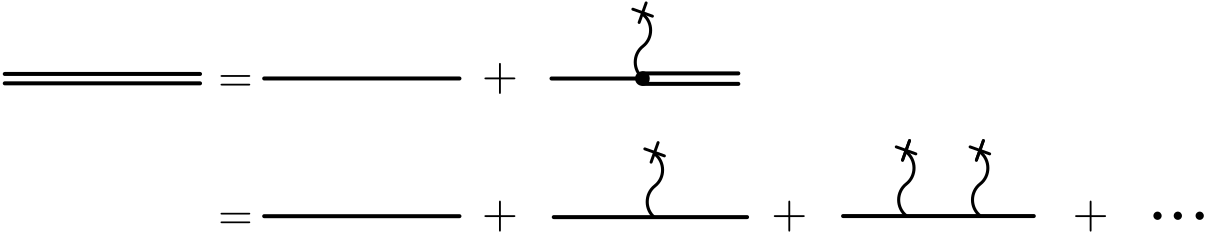
\includegraphics[width=0.9\linewidth]{pics/propagator.pdf}%
\caption{Relation between the propagator including the external field and the propagator of the free theory in Feynman diagrams corresponding to Eq.~\eqref{eq:propeq}. A double line corresponds to the dressed propagator in the external field, a single line to the free Dirac propagator, and a wave line with a cross to the interaction with the external field. The propagator in the external field is obtained by including all interactions with the external field in the free propagator.}%
\label{fig:propagator}%
\end{figure}
%
Another useful form of the Propagator in the external field is the spectral representation in terms of the Dirac wave functions~\eqref{eq:wavefct}. By inserting a complete set of states in Eq.~\eqref{eq:extpropdef}, one obtains
\begin{equation}
S_\mathcal{A}(x,y)=\Theta(x^0-y^0) \sum_n u_n(x)\bar{u}_n(y)
-\Theta(y^0-x^0)\sum_m v_m(x)\bar{v}_m(y).
\end{equation}
For a time-independent external field, a Fourier transformation in the zeroth component yields
\begin{equation}
\tilde{S}(\mathbf{x},\mathbf{y},E)= \sum_n \frac{u_n(\mathbf{x})\bar{u}_n(\mathbf{y})}{E_n -E -i\,\epsilon}
+\sum_m \frac{v_m(\mathbf{x})\bar{v}_m(\mathbf{y})}{E_m +E -i\,\epsilon}.
\label{eq:spectralrep}
\end{equation}
Therefore, bound states due to the external field lead to additional isolated poles in the propagator.

\subsubsection*{Propagator of interacting theory}
Finally, we will consider the propagator in the interacting theory, including the interaction with the quantized photon field. A similar argument as in the derivation of Eq.~\eqref{eq:spectralrep} also holds for the interacting theory~\cite[Section 14.2.]{weinberg2005}. This is, bound state energies including all radiative corrections appear as isolated poles of the full propagator. In order to locate the positions of these poles, perturbation theory with the propagator including the external field is used, expanding the propagator in powers of the finestructure constant $\alpha=e^2/(4\pi)$. The zero-order term is the dressed propagator in the background field, corresponding to solving the Dirac equation with the background field. The diagrams contributing to the radiative corrections to first order in $\alpha$ are the vacuum-polarization~(VP)and self-energy~(SE) diagrams shown in Fig.~\ref{fig:1loop} $(a)$ and $(b)$, respectively. Using the Feynman rules~\mbox{\cite[Section 6.1.]{itzykson2005}}, the propagator of the interacting theory $S_{I}(x,y)$ is expanded to first order in $\alpha$ as
\begin{alignat}{2}
&S_{I}(x,y) &&\approx S_{\mathcal{A}}(x,y) + \int \mathrm{d}^4z_1\,\mathrm{d}^4z_2\,
S_{\mathcal{A}}(x,z_1)\,\left[\Sigma_{\text{VP}}(z_1,z_2)+\Sigma_{\text{SE}}(z_1,z_2)\right]\,S_{\mathcal{A}}(z_2,y),\notag\\
&\Sigma_{\text{VP}}(z_1,z_2)&&=-\delta(z_1-z_2)(-ie\gamma^\mu)\int \text{d}z\,S_P(z_1-z)\Tr ((-ie\gamma_\mu)S_{\mathcal{A}}(z,z)),\notag\\
&\Sigma_{\text{SE}}(z_1,z_2)&&=(-ie\gamma^\mu)S_{\mathcal{A}}(z_1,z_2)S_P(z_1-z_2)(-ie\gamma_\mu),
\end{alignat}
where $g_{\mu\nu}S_P(x-y)$ is the photon propagator in position space~\mbox{\cite[Section 3.2.]{itzykson2005}}. Using the Fourier transformed functions
\begin{equation}
\Sigma_{\text{VP/SE}}(\mathbf{z}_1,\mathbf{z}_2,E)= \int \text{d}z_1^0\, \e^{iE(z_1^0-z_2^0)}\Sigma_{\text{VP/SE}}(z_1,z_2),
\end{equation}
and the spectral representation of the propagator from Eq.~\eqref{eq:spectralrep}, it can be shown~\mbox{\cite[Section 14.2.]{weinberg2005}} that the levelshifts of the $n$-th level read as
\begin{equation}
\Delta E_n = \int \text{d}^3\mathbf{x}\,\text{d}^3\mathbf{y}\,\bar{u}_n(\mathbf{x})\left( -\Sigma_{\text{VP}}(\mathbf{x},\mathbf{y},E_N)-\Sigma_{\text{SE}}(\mathbf{x},\mathbf{y},E_N) \right)u_N(\mathbf{y})
\end{equation}

%
\begin{figure}%
\centering
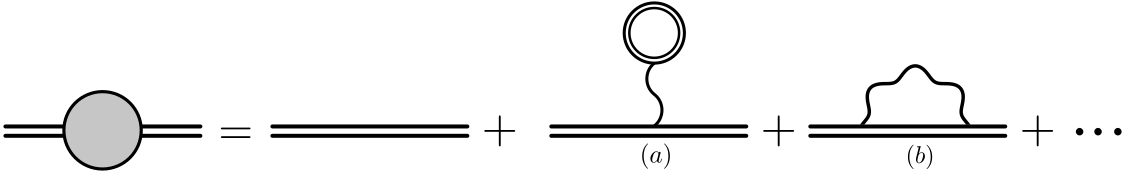
\includegraphics[width=0.9\linewidth]{pics/1loop.pdf}%
\caption{Perturbative expansion of the propagator of the interacting theory in powers of~$e^2$. The zero-order contribution is the propagator in the external field. To first order in~$e^2$, the contributions are the vacuum-polarization diagramm~$(a)$ and the self-energy diagram~$(b)$.}%
\label{fig:1loop}%
\end{figure}
%


\subsection{Vacuum polarization potentials}
%
\begin{figure}%
\centering
\includegraphics[width=0.9\linewidth]{pics/vac_pol.pdf}%
\caption{Top row: Expansion of the order $\alpha$ vacuum polarization in powers of $(Z\alpha)$, in which the contributions with odd powers vanish. The $\alpha(Z\alpha)$ contribution (diagram $a$) is the Uehling term, the $\alpha(Z\alpha)^3$ contribution (diagram $b$) is the Wichmann-Kroll term. \\Bottom row: Contributions to the Källen-Sabry terms (diagrams $c$-$f$) of order $\alpha^2(Z\alpha)$.}%
\label{fig:vac_pol}%
\end{figure}
%
\section{Dirac equation in central potentials}
...
\subsection{Solution of the Coulomb problem}
...
\subsection{Numerical solution in a cavity}






